\documentclass[
	12pt,
	a4paper,
	twoside,
	english,
	headsepline,
	footnosepline,
	automark,
	normalheadings,
	openany,
	cleardoubleplain,
	abstracton,
	idxtotoc,
	liststotoc,
	bibtotoc,
 	BCOR8mm,
]{scrartcl}

\usepackage{
	calc,
	color,
	fancybox,
	fancyvrb,
	float,
	mdwlist,
	scrdate,
	scrtime,
	scrpage2,
	tabularx,
	ucs,
	multirow
}

\usepackage[utf8x]{inputenc}

\usepackage{graphicx}
\graphicspath{{img/}}
\usepackage{hyperref}
\usepackage{listings}

\pagestyle{scrheadings}
\setkomafont{pagehead}{\small\scshape}
\setcounter{tocdepth}{3}

\newcommand{\dctitle}{B.A.T.M.A.N. Daemon HowTo}
\newcommand{\dcsubject}{~}
\newcommand{\dcauthorlastname}{Tsai}
\newcommand{\dcauthorfirstname}{Wesley}
\newcommand{\dcauthoremail}{wesleyboy42(AT)gmail(DOT)com}
\newcommand{\dcdate}{\today}

\hypersetup{
	pdftitle	= {\dctitle}, %
	pdfsubject	= {\dcsubject, \dcdate}, %
	pdfauthor	= {\dcauthorfirstname~\dcauthorlastname, \dcauthoremail}, %
	pdfkeywords	= {mesh}, %
	pdfcreator	= {pdfTeX with Hyperref}, %
	pdfproducer	= {LaTeX, hyperref, thumbpdf}, %
	colorlinks=false, %
	linkbordercolor= {1 1 1}, %
}
\title{\dctitle}
\author{\dcauthorfirstname~\dcauthorlastname}

\newcommand{\subsubsectionttt}[1]{\subsubsection{\texttt{#1}}}

\fussy
\begin{document}
\maketitle

\begin{abstract}
B.A.T.M.A.N stands for ``better approach to mobile ad hoc networking'', this is
a new routing protocol for multi-hop ad-hoc mesh networks. Go to
\url{http://www.open-mesh.net} to see more information.

The following document will explain how to install and use the B.A.T.M.A.N.
daemon.
\end{abstract}


\section{Installing from source}
\subsection{Prerequirements}

\begin{itemize}
 \item Compile environment and libraries.
       \begin{enumerate}
        \item gcc
        \item libc6-dev
        \item build-essential
        \item binutils
        \item makedev
        \item GNU make
        \item libpthread
       \end{enumerate}
\item Download the B.A.T.M.A.N. daemon code from the website

     \url{http://www.open-mesh.net/wiki/Download}
\end{itemize}


\subsection{Compiling}
All you have to do is untar and make, then you will see the executable file
called \emph{batmand}.

{\footnotesize
\begin{verbatim}
 $ wget \
http://downloads.open-mesh.net/batman/stable/sources/batman/batman-0.3.tar.gz
 $ tar xzvf batman-0.3.tar.gz
 $ cd batman-0.3
 $ make
\end{verbatim}
}

If you want reduce the size of executable file, just strip it by executing: 

\begin{verbatim}
 $ strip batmand
\end{verbatim}

Note that if you want to help us finding a bug in the daemon, please don't strip
it.

\subsection{Installing}
Copy \emph{batmand} to a location somewhere in your path, for example
\begin{verbatim}
 $ cp batmand /usr/sbin/
\end{verbatim}
Or start it right from the directory where you compiled it
\begin{verbatim}
 $ ./batmand
\end{verbatim}


\section{Usage}
If you execute \verb+batmand -h+ or \verb+-H+, you will see the help page, in
the following we will explain all parameters and how to work with them in a mesh
network.

\subsection{SYNOPSIS}
\begin{verbatim}
batmand [options] interface [interface...]
\end{verbatim}


\subsection{DESCRIPTION}
You can start batmand without specifying options, but you have to choose at
least one interface batmand runs on.
\begin{verbatim}
 $ batmand eth1
\end{verbatim}
If you have more interfaces, then you just add them behind the first.
\begin{verbatim}
 $ batmand eth1 eth2 eth3
\end{verbatim}
The B.A.T.M.A.N. daemon can also run on alias interfaces. Note that we use alias
interfaces to separate B.A.T.M.A.N. routing protocol and olsr routing protocol.
\begin{verbatim}
 $ batmand eth1:test1 eth2:test2 eth3:test3
\end{verbatim}
Note that the B.A.T.M.A.N. daemon will take the ip address and the broadcast
address from the given interfaces.

Note also that you have to check whether your essid, channel or wifi mode is
correct or not.

\subsubsectionttt{-a add announced network(s)}
The daemon announces the availability of a connection to another network. This
option can be used multiple times and can be used to add networks dynamically
while the daemon is running. The parameter has to be in the form of
ip-address/netmask.

For example, if you are the node A, and you can connect to \emph{other
network}, then you can execute a to announce the gateway.

\begin{center}
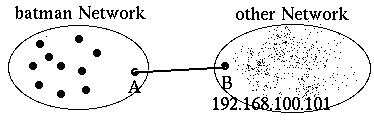
\includegraphics[scale=0.8]{announce_networks}
\end{center}

If the other nodes in the B.A.T.M.A.N. network want to connect to node B after
receiving the announce network information form node A, then they will know they
can use node A as gateway to reach node B. Now, you know what a announced
network is, but executing this command is wrong:
\begin{verbatim}
 $ batmand -a 192.168.100.101 eth1
\end{verbatim}

Because you have to specify the netmask parameter and different netmask
parameters cause different results. Let's make a example:
\begin{verbatim}
 $ batmand -a 192.168.100.101/32 eth1
\end{verbatim}
In this case, it means that node A can only connect to node B, because your
parameter is /32.

\begin{verbatim}
 $ batmand -a 192.168.100.101/24 eth1
\end{verbatim}
In this case, it means that node A can connect to the whole 192.168.100.x
network, because your parameter is /24. So, if you use different netmask values,
then the results are different.

\begin{center}
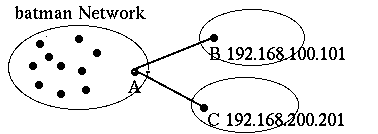
\includegraphics[scale=0.8]{multiple_announces}
\end{center}

Node A can announce more than one network. To announce two networks execute the
following command:
\begin{verbatim}
 $ batmand -a 192.168.100.101/24 -a 192.168.200.201/24 eth1
\end{verbatim}
Note that node A has to have a route to connect the node or network.

\subsubsectionttt{-A delete announced network(s)}
Delete networks to the daemons list of available connections to another
network(s). This option can be used multiple times and can only be used while
the daemon is running. The parameter has to be in the form of
ip-address/netmask.

\subsubsectionttt{-b run connection in batch mode}
The debug information are updated after a period of time by default, so if you
use "-b" it will execute once and then stop.
\begin{verbatim}
 $ batmand eth1
 $ batmand -b -c -d 1
\end{verbatim}
In this case, it means run debug level 1 once.

Note that -b can only be used with -c and debug level 1 \& 2.

\subsubsectionttt{-c connect via unix socket}
The B.A.T.M.A.N. daemon offers a unix socket interface to which you can connect.
First, you have to create a B.A.T.M.A.N. daemon on your host, then use -c to
connect to its interface. Note you can create as many client sockets as you
like.
Deploy it without any arguments to get the current configuration even if changed
at runtime.

\begin{center}
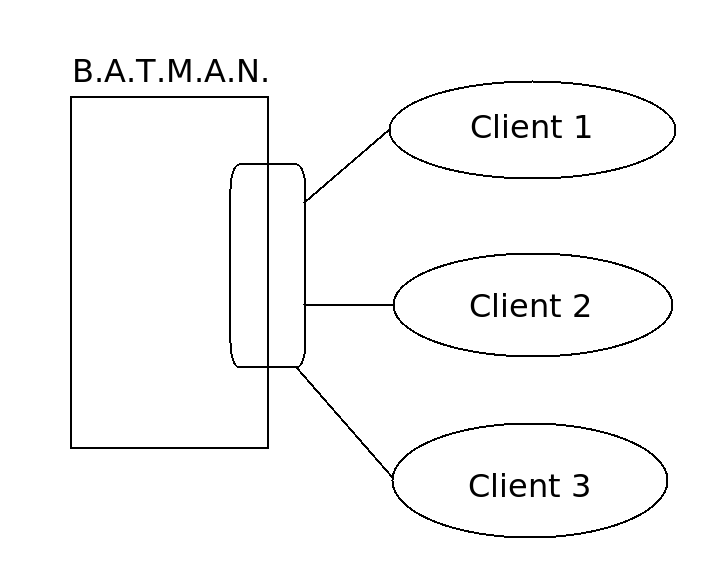
\includegraphics[scale=0.5]{multiple_clients}
\end{center}

\begin{verbatim}
 $ batmand eth1
 $ batmand -c -d 1
\end{verbatim}
In this case, you ask the daemon to output debug level 1 in your current shell.
The B.A.T.M.A.N. daemon will update the information after a period of time.

Note that if you use -c flag, then you only can use -d to see the debug level.

\subsubsectionttt{-d debug level}
The debug level can be set to five values.

\begin{description}
 \item[0] debug disabled (default)
 \item[1] list neighbors
 \item[2] list gateways
 \item[3] observe batmand
 \item[4] observe batmand (very verbose)
 \item[5] memory debug / cpu usage
\end{description}
Note that debug level 5 can be disabled at compile time.

For example, you can run in normal start:
\begin{verbatim}
 $ batmand -d 1 eth1
\end{verbatim}

\paragraph*{Level 1}
just lists the neighbors in your B.A.T.M.A.N. network.

\begin{lstlisting}[basicstyle=\footnotesize,	frame=single, columns= flexible]
Originator      Router (#/128):       Potential routers... [B.A.T.M.A.N. 0.2, MainIF/IP:
eth2 105.131.131.175, UT: 0d 0h 3m]
105.131.83.2    105.131.1.3 (  71):   105.131.1.3 (  71)
105.131.1.2     105.131.1.2 (  52):   105.131.1.2 (  52)
105.131.56.10   105.131.1.4 (  25):   105.131.1.4 (  25),105.131.1.6 ( 15), 105.131.1.7 ( 10),..
105.131.131.70  105.131.131.70 (121): 105.131.131.70 (121)
\end{lstlisting}

\begin{itemize}
\item In the first line, we will see the version of the B.A.T.M.A.N. daemon,
      main interface, main IP, and uptime.
\item In the first column, we can see those IPs which we can reach.
\item In the second column, we can see those IPs which we sent our packets to
      when we want to reach the IP of the first column. The number in the
      parenthesis indicates the link quality of the connection and the
      \verb|#/128| shows the maximum number of packets.
\item In the third column, we can see those IPs which are one hop neighbors and
      rebroadcasted packets from the originator. The B.A.T.M.A.N. daemon will
      choose the router with the best link quality from the potential router
      list.
\end{itemize}

In this case, 105.131.1.2 is a one hop neighbor of 105.131.131.175, because the
105.131.1.2 is originator, router and potential router at the same time. If
105.131.131.175 wants to exchange data with the 105.131.83.2, then it will sent
its packets to the 105.131.1.3, because it is the router for this destination.

\paragraph*{Level 2}
just lists gateways in the B.A.T.M.A.N. network.

\begin{lstlisting}[basicstyle=\footnotesize,	frame=single, columns= flexible]
Gateway         Router (#/128)
105.131.83.5    105.131.41.1 ( 57), gw_class 11  ->6 MBit, reliability: 0
105.131.41.5    105.131.41.1 ( 53), gw_class 11  ->6 MBit, reliability: 0
\end{lstlisting}

\begin{itemize}
\item In the first column, we can see those IPs which are our gateways.
\item In the second column, we can see those IPs which we sent our packets to
      when we want to reach the IP of the first column. The number in the
      parenthesis indicates the link quality of the connection and the
      \verb|#/128| shows the maximum number of packets. The \verb|gw_class|
      means gateway class of the gateway and \verb|11 ->6 MBit| means how much
      bandwidth the gateway owner wants to share. The reliability means how good
      the quality of the internet connection is. In this case, \verb|0| means
      this is the best quality. The reliability number will increase if the
      quality is poor.
\end{itemize}

\paragraph*{Level 3}
has more information about the neighbors, or shows the error message when you
have an incorrect command. Note that if there is no neighbor in the B.A.T.M.A.N.
network, then it will display nothing.

\paragraph*{Level 4}
has so many information about the B.A.T.M.A.N. network, for example, how many
packets you sent, and sent to where, or how many packets you got, and received
from where etc.

\subsubsectionttt{-g gateway class}
The gateway class is used to tell other nodes in the network your available
internet bandwidth. Just enter any number (optionally followed by "kbit" or
"mbit") and the daemon will guess your appropriate gateway class. Use "/" to
seperate the down- and upload rates. You can omit the upload rate and batmand
will assume an upload of $\mathrm{download}\over{5}$.

\begin{itemize}
\item 5000
\item 5000kbit
\item 5mbit
\item 5mbit/1024
\item 5mbit/1024kbit
\item 5mbit/1mbit
\end{itemize}
You only can set the value in a normal start
\begin{verbatim}
 $ batmand -g 5mbit/1024 -d 3 eth1
\end{verbatim}
Note that if you use debug level 3, then you will know whether you succeed
setting the gateway class or not.

\subsubsectionttt{-o originator interval in ms}
A node transmits broadcast messages (we call them originator message or OGM) to
inform the neighboring nodes about it’s existence. Originator interval is the
time to wait after sending one message and before sending the next message.
The default value is 1000 ms (1 second). In a mobile network, you may want to
detect network changes very quickly, so you need to send message very often, for
example, use a value of 500 ms. In a static network, you can save bandwidth by
using a higher value. This option is only available in daemon mode.
\begin{verbatim}
 $ batmand -o 2000 eth1
\end{verbatim}
In this case, batmand will wait 2 second until sending the next OGMs.

\subsubsectionttt{-p preferred gateway}
Set the internet gateway by yourself. 

Note that this automatically switches your B.A.T.M.A.N. daemon to "internet
search modus" with "-r 1" unless "-r" is given. If the preferred gateway is not
found the gateway selection will use the current routing class to choose a
gateway.

\begin{verbatim}
 $ batmand -r 3 -d 3 -p 192.168.1.1 eth1
\end{verbatim}
In this case, you set 192.168.1.1 as your preferred gateway, so all of your
internet packets will be sent to the 192.168.1.1.

\subsubsectionttt{-r routing class}
The routing class can be set to four values - it enables "internet search
modus". The daemon will choose an internet gateway based on certain criteria
(unless "-p" is specified):
\begin{description}
\item[0] set no default route (default)
\item[1] use fast connection
\item[2] use stable connection
\item[3] use fast-switch connection
\item[XX] use late-switch connection
\end{description}

\paragraph*{Level 1}
B.A.T.M.A.N tries to find the best available connection by watching the uplinks
throughput and the link quality.

\paragraph*{Level 2}
B.A.T.M.A.N compares the link quality of the internet node and chooses the one
with the best connection.

\paragraph*{Level 3}
B.A.T.M.A.N compares the link quality of the internet node and chooses the one
with the best connection but switches to another gateway as soon as a better
connection is found.

\paragraph*{Level XX}
B.A.T.M.A.N compares the link quality of the internet node and chooses the one
with the best link quality but switches to another gateway as soon as this
gateway has a TQ value which is XX better than the currently selected gateway.

XX ist a number between 3 and 256

\begin{verbatim}
 $ batmand -r 3 -d 3 eth1
\end{verbatim}
In this case, the B.A.T.M.A.N. daemon will choose the best statistic internet
connection for you. Note that if you use debug level 3, then you will know
whether you succeeded setting the routing class or not.

\subsubsectionttt{-s visualization server}
Since no topology database is computed by the protocol an additional solution to
create topology graphs has been implemented, the vis server. B.A.T.M.A.N.
daemons may send their local view about their single-hop neighbors to the vis
server. It collects the information and provides data in a format similar to
OLSR's topology information output. Therefore existing solutions to draw
topology graphs developed for OLSR can be used to visualize mesh-clouds
using B.A.T.M.A.N.

\subsubsectionttt{--policy-routing-script}
This option disables the policy routing feature of batmand - all routing changes
are send to the script which can make use of this information or not. Firmware
and package maintainers can use this option to tightly integrate batmand into
their own routing policies. This option is only available in daemon mode.


\section{Reference Links}
\begin{itemize}
\item \url{http://www.open-mesh.net/}
\item \url{http://www.olsr.org/}
\end{itemize}

\section{Troubleshooting}
\subsection{Why the B.A.T.M.A.N. daemon doesn't reload the setting after I fixed the main IP?}
You have to restart the B.A.T.M.A.N. daemon after you modified any network
configuration, otherwise the B.A.T.M.A.N. daemon won't use the new settings.
\begin{verbatim}
 $ killall batmand
 $ batmand eth1
\end{verbatim}

\subsection{Why I can't connect to the Internet after setting the default gateway?}
You have to use NAT on your gateway or firewall if you use the -r or -p options
to set default route.
\begin{verbatim}
 $ iptables -t nat -A POSTROUTING -o eth1 -j MASQUERADE
\end{verbatim}
Note that you don't set the default route by yourself.

\vfill
\section*{Copyright}
\begin{center}
 
\includegraphics[scale=0.8]{byncsa30}
\end{center}
This work is licensed under the Creative Commons Attribution-Noncommercial-Share
Alike 3.0 License. To view a copy of this license, visit
\url{http://creativecommons.org/licenses/by-nc-sa/3.0/} or send a letter to
Creative Commons, 559 Nathan Abbott Way, Stanford, California 94305, USA.
\end{document}
